

\begin{figure}
  \centering
  
\includegraphics[scale=0.18]{images/data_pipeline.pdf}
  \caption{Yi's pretraining data cleaning pipeline. 
  % \alex{Change ``security'' to ``safety''. In principle we should always use ``safety'' over ``security'' because ``security'' is geo-politically indicating, e.g., ``national security''}\alex{Also TODO: add ``cluster-based filtering''}
  }
  \label{fig:data_cleaning}
\end{figure}
% The pretraining stage sets the foundation of the comprehensive abilities of LLMs~\citep{zhao2023survey}, as it embeds essential factual associations of the world~\citep{meng2022locating}, and cultivates advanced capabilities such as arithmetical operations~\citep{azerbayev8llemma}, coding~\citep{roziere2023code}, logical reasoning~\citep{pan2023logic,yue2023mammoth}, and policy learning~\citep{feng2023chessgpt,li2022emergent}. In this section, we provide a comprehensive preview of the pretraining stage of Yi, encompassing introductions to the dataset, tokenization, and model architecture.

Our approach to pretraining is to train a standard dense transformer architecture on a heavily engineered large pretraining corpora, where our underlying assumption is that when trained on extensive data of high-enough quality, a standard architecture can exhibit advanced capability. 
This is to say, we may not need much architectural modification, although we have indeed conducted extensive preliminary architectural experiments. 
In the following subsections, we first detail our data engineering pipeline, then briefly discuss the model architecture. 

\subsection{Data Processing}

% Briefly Explain the data sources, detailedly explain the data processing procedure.
% A sketch map is introduced to describe the data processing pipeline(Todo) 
% Recent study of LLM scaling law \citep{Hoffmann:2022aa} encourages an increasing focus on training dataset scaling, and hence we created a massive bilingual corpus of 3 trillion high quality tokens for 01ai pretraining. 
%The 01ai corpus is composed of multiple sources: web documents, encyclopedias, question answers, books, codebases, academic papers, and instruction data. 
% In the data mixture, English : Chinese : code ratio is 72.3 : 19.2 : 8.5.

% High-quality pretraining data is widely acknowledged as a pivotal factor in the success of training LLMs~\citep{gao2020pile,DolmaDataset,penedo2023refinedweb,shen2023slimpajamadc}. 
% Nonetheless, the integration of filtered web data with specialized datasets like books, technical papers, instructions, and encyclopedic content poses significant challenges~\citep{penedo2023refinedweb}, particularly when developing bilingual LLMs for Chinese and English. These challenges have yet to be thoroughly investigated. To tackle these issues, we have formulated a comprehensive empirical methodology for compiling reliable bilingual pretraining data. This methodology is tailored to facilitate cutting-edge research in bilingual LLM technology.
% Our approach includes a meticulously designed cascaded data-cleaning strategy, 

The Yi data mixture is shown in Fig.~\ref{fig:data_mixture}.
To produce a high-quality bilingual pretraining data, 
we meticulously designed a cascaded data-processing pipeline, as illustrated in Fig~\ref{fig:data_cleaning}. 
This pipeline features a series of data-cleaning strategies targeting  quality and diversity. 
We start with web documents from Common Crawl, use the CCNet pipeline \citep{Wenzek:2019aa} for language identification and perplexity  scoring. 
Then we use a combination of filtering and deduplication process, as detailed below. 

% Importantly, this method is highly adaptable, enabling customization to accommodate the diverse characteristics of raw data sourced from various origins.


% Nota bene that the data-cleaning pipeline is\qj{can be} moderately manipulated to suit the different conditions of raw data from different data sources. 

\paragraph{Heuristic Rule Filters} 
This part of filter aims for removing text of low quality. 
We filter out text based on: 
(1). URL, domain, word blocklists and garbled text filters; 
(2). document length, the ratio of special symbols, and the ratio of short, consecutive, or incomplete lines;
(3). repeated words, n-grams, or paragraphs \citep{rae2021scaling};
The filtering thresholds are based on a statistical analysis of large document samples, as described in \citet{nguyen2023culturax}. 
% We employ a multi-faceted approach that includes the use of URL/domain blocklists, word blocklists, and garbled text filters. 
% Our strategy targets the elimination of low-quality Web documents, employing key text metrics such as document length, the ratio of special symbols, and the ratio of short or incomplete lines. 
% The filtering thresholds are determined based on statistical analysis of a vast corpus of document samples, as delineated in \citet{nguyen2023culturax}. 
% Additionally, our methodology entails the removal of documents exhibiting a high frequency of repeated words, n-grams, or paragraphs \citep{rae2021scaling}, as well as those with consecutive short lines, which are often indicative of irrelevance to the core content. 
Furthermore, we identify and anonymize Personal Identifiable Information (PII), such as email addresses and phone numbers.

\begin{wrapfigure}{r}{0.5\textwidth}
	\begin{center}
		\vspace{-0.3in}
		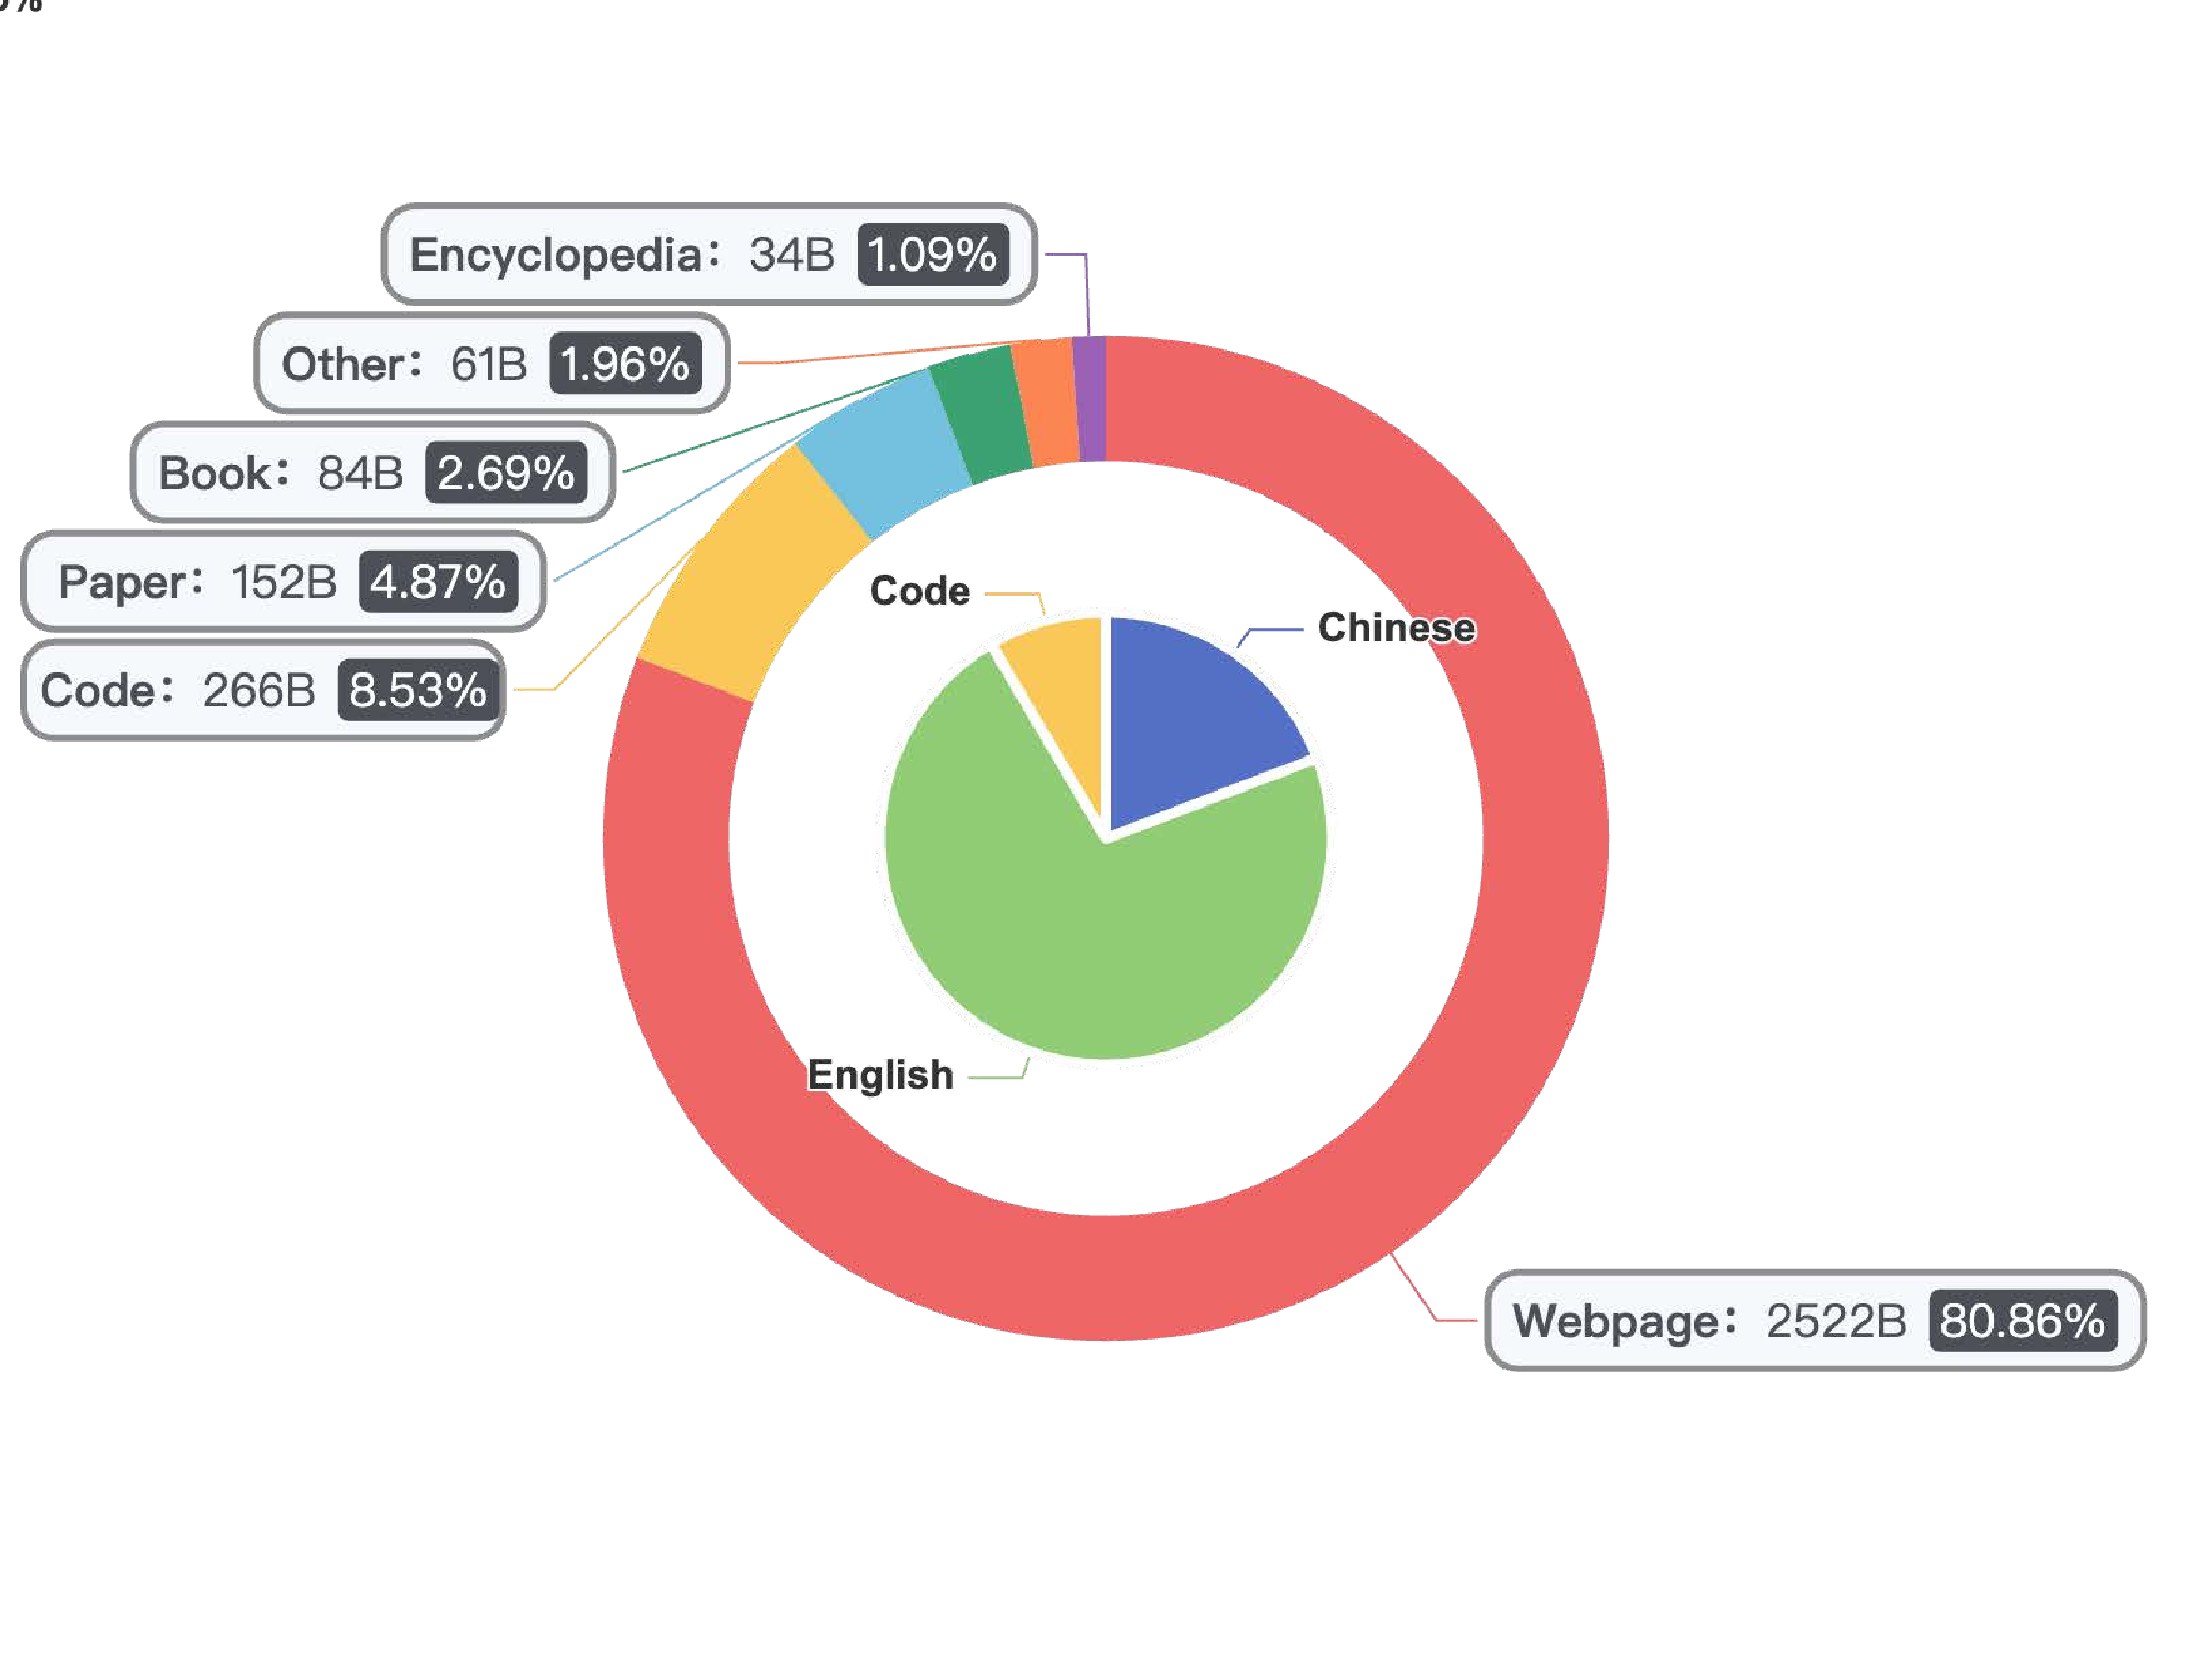
\includegraphics[width=0.5\textwidth]{images/data_mixture.pdf}
	\end{center}
	\vspace{-0.15in}
	\caption{Yi's pre-training data mixture. Overall our data consist of 3.1T high-quality tokens in Both English and Chinese, and come from various sources. Our major differences from existing known mixtures like LLaMA~\citep{touvron2023llama} and Falcon~\citep{penedo2023refinedweb} are that we are bilingual, and of higher quality due to our more rigorous cleaning pipeline.} %
	\label{fig:data_mixture}
    \vspace{-0.2in}
\end{wrapfigure}
\paragraph{Learned Filters} 

We use learned filters to address nuanced cases that exceed the capabilities of standard heuristic rules. Notably, the Chinese content extracted from Common Crawl present unique challenges, particularly with a higher ratio of inappropriate content like pornography and gambling. Traditional heuristic-rule-based filters struggle to effectively identify and eliminate all harmful content. To enhance our filtering process, we have integrated a suite of learned scorers for filtering, namely the perplexity scorer, quality scorer, safety scorer, and document coherence scorer:
(1). the \textit{Perplexity Scorer}, utilizing the KenLM library as per CCNet \citep{wenzek2019ccnet}, evaluates a vast array of web documents, discarding those with perplexity scores largely above average;
(2). the \textit{Quality Scorer} is a classifier trained to recognize and favor pages similar to Wikipedia in quality and assign scores accordingly. Documents that fail to meet the quality standard are subsequently removed;
(3). the \textit{Document Coherence Scorer} identifies low-quality web documents that consist of disparate sentences or paragraphs, thus being incoherence. Such documents are either segmented for further analysis or removed entirely. 
(4). the \textit{Safety Scorer} identifies and removes web documents containing toxic content, such as violence, pornography, and political propaganda.

\paragraph{Cluster-based Filters} 
% To facilitate the retrieval of similar documents for both automatic and manual data quality verification, 
We further use unsupervised semantic clustering to group web documents. This clustering process enables efficient identification and analysis of documents sharing similar semantic features. The clustered data are subsequently annotated with quality labels, providing essential references for the optimization of Yi's data mixture strategy. Documents identified as low-quality through automatic and manual verification are excluded from the dataset.

\paragraph{Deduplication} 
After filtering, we implement a comprehensive deduplication pipeline following the procedure in Penedo et al. (2023) \citep{penedo2023refinedweb}. This pipeline integrates document-level MinHash deduplication and sub-document exact-match deduplication, effectively identifying and removing duplicate content within and across documents. We further categorize web documents into specific themes using a topic model predicting labels like as news, ads, and knowledge-based content. In the final pretraining dataset, we down-sample less helpful content, mostly advertisements, to ensure information density. The final composition of Yi's pretraining data  is shown in Fig.~\ref{fig:data_mixture}.


\subsection{Tokenization}
We use byte-pair encoding (BPE)~\citep{shibata1999byte} implemented in the SentencePiece framework~\citep{kudo2018sentencepiece}, to tokenize the pretraining data.
The vocabulary size of Yi is set to 64,000 to balance computational efficiency and word comprehension.
% \alex{Did we try 128000 and why not using it?}
Specifically, we split numbers into individual digits to facilitate a better understanding of numeric data.
We allow rare characters to fall back to the unicode-byte encoding to ensure fault tolerance.
We employ the identity tokenizer to avoid transferring all punctuations to the half-width format.
LLMs prioritizing English usually utilize dummy prefix (whitespace at the beginning of text) in their tokenizers to generalize the same words at different positions of sentences.
We do not use this approach because the assumption does not always hold even in the English context, especially for sentences that begin with quotation marks, also it does not show positive effect in Chinese context.
% In contradiction with LLMs prioritizing English, we do not add dummy prefixes.\xy{This sentence and the following one sound not clear to me. What are dummy prefixes? We might either give a reference or explain it shortly. }
% Because there are no spaces as separators in Chinese grammar, there is no need to introduce the dummy prefix to generalize the same words at the beginning and the middle of sentences.
% \qj{add explanations for how to deal with English texts or why dummy prefixes are not necessary for English as Yi is a bilingual LLM?}

\subsection{Model Architecture}
\begin{table}[t!]
    \centering
    \begin{tabular}{@{}cccccccc@{}}
        \toprule
         Models&  Hidden Size&  Q-heads&  KV-heads&  Layers&  Pretrain Seq. Len& Max LR\\
         \midrule
         6B&  4096&  32&  4&  32&  4096& $3\times10^{-4}$\\
         34B&  7168&  56&  8&  60&  4096& $1.5\times10^{-4}$\\
         \bottomrule
    \end{tabular}
    \space
    \caption{Model configs of Yi-6B and Yi-34B. LR stands for learning rate.}
    \label{tab:model_config}
\end{table}
Yi uses a modified version of the classical decoder-only Transformer architecture~\citep{Vaswani:2017aa} where the code is based on LLaMA's~\citep{llama2} implementation. 
The main parameter setting is summarized in Table~\ref{tab:model_config}. 
%We also introduce a few changes, which we summarize below.
The modifications from LLaMA to Yi are further summarized below:

\paragraph{Attention Mechanism} LLaMA 2 uses Grouped-Query Attention(GQA)~\citep{gqa} only on its largest 70B model, and its 7B and 13B uses full attention. We incorporate GQA in both Yi-6B and Yi-34B. 
GQA splits query-heads into G groups, sharing a single key and value head within each group of query~\citep{gqa}.
This approach offers substantial reductions of training and inference costs, compared to the original Multi-Head Attention (MHA)~\citep{shazeer2019fast,de2022fido,pope2023efficiently}.
We do not observe performance degradation after applying GQA to our 6B smaller model. 

% Although the L\textsmaller{LaMA} 2 series models only implemented GQA in the L\textsmaller{LaMA} 2-70B, we demonstrate that the adoption of GQA does not result in noticeable performance degradation in our model.

\paragraph{Activation Function} 
We use SwiGLU~\citep{swiglu} as Yi's post-attention layer, reducing its activation size from $4h$ to $8/3h$ ($h$ denotes hidden size) to be consistent with the normal post-attention layer. 
% We employ SwiGLU~\citep{swiglu} as Yi's post-attention layer, strategically fine-tuning the hidden size to optimize throughput within our infrastructure. 
This adjustment also compensates for the reduction in parameter resulted from GQA, making the overall parameter count comparible of existing 7B and 34B models. 

% This meticulous adjustment not only compensates for the reduction in parameter count resulting from the integration of GQA but also ensures that the overall model parameters align closely with both the 6B and 34B.

\paragraph{Positional Embedding and Long Context}
% Rotary Position Embedding (\textbf{RoPE})~\citep{su2021roformer}, a demonstrated and widely-used position embedding, is selected to incorporate positional information into Yi-6B and Yi-34B.
% Specifically, we utilize the RoPE with adjusted base frequency (\textbf{RoPE ABF})~\citep{xiong2023effective} in Yi-6B and Yi-34B to support effective context windows up to \textcolor{red}{detailed number here} and BF16 precision to accelerate the pretraining procedure.
% We further propose a two-stage empirical pretraining plan adapting RoPE ABF to empower a longer reliable context window, which is illustrated in Sec.~\ref{sec: context length}.

% Rotary Position Embedding (\textbf{RoPE})~\citep{su2021roformer}, a well-established and widely used method to incorporate positional information, has been chosen to integrate positional information into Yi-6B and Yi-34B. Specifically, 
We use Rotary Position Embedding 
 (RoPE)~\citep{su2021roformer} following the standard implementation.
We adjust the base frequency (RoPE ABF), introduced in~\citet{xiong2023effective}, to support long context windows up to 200K where the base model itself is trained on 4K context length. 
To adapt the base model to longer context, we continue pretrain the model on 10B tokens from our pretraining data mixture with slightly upsampled long sequences, mostly from book. 
We observe that only 1-2B tokens is enough for the model to converge to low loss on 4K-200K length, and a lightweight finetuning further induces near-perfect long-context retrieval performance. 
Based on this observation, we tend to view that the capability of modeling longer dependency than the pretrained length (4K) is a intrinsic capability (rather than an being injected by post-train).
This is to say, the base model already has the capability to model longer than 4K dependency even the model is trained shorter, and the post-train / finetuning procedure simply release this capability.


% \paragraph{Group Query Attention (GQA) \citep{gqa}.} In contrast to Llama2, we incorporate GQA in both the 6B and 34B versions of Yi. 
% We observe that the utilization of GQA does not result in any noticeable performance degradation. 
% However, it does offer substantial reductions in training and inference costs. 

% \paragraph{SwiGLU}\citep{swiglu}. We utilize SwiGLU as Yi's post-attention layer, reducing its hidden size from 4 to $\frac{8}{3}$ to be consistent with the normal post-attention layer. 
% The inclusion of GQA significantly decreases Yi's parameter size.
% As a result, to maintain Yi's capability, we multiply the intermediate hidden layer used by SwiGLU, bringing our model reasonably close to 6B and 34B.
% \textcolor{Red}{[To Polish.]}
% This reduction significantly decreases Yi's parameter size as a result of the inclusion of GQA. 
% To maintain the model's capability, we multiply the intermediate hidden layer used by SwiGLU, bringing our model reasonably close to 6B and 34B.